\chapter{Query Language}\label{sec:specification_language}

The SMT-LIB language is a well-known language used to formalize 
Satisfiability Modulo Theories problems, and is expressive enough to
represent the verification properties of interest. In this language, 
it is possible to define both the \textit{pre-} and 
\textit{post-}conditions at once, by defining the variables for the
input and the output of the neural network. In the following we
show some examples of networks and corresponding properties in the
SMT-LIB language.

\section{Syntax}
\label{sec:syntax}

The syntax of VNN-LIB is formally defined using Labelled Backus-Naur Form (LBNF)\cite{8}. LBNF is a variant of BNF that allows for 
annotations (labels) on productions, facilitating the automatic generation of abstract syntax trees, parsers, and other language processing tools. 
This formal grammar provides a rigorous foundation for the language, eliminating ambiguities present in previous versions and ensuring consistent 
parsing across different tools.

The full LBNF grammar for VNN-LIB is provided in the Appendix~\ref{app:lbnf_grammar}. The following subsections highlight key syntactic constructs of the language,
with examples illustrating their usage.

\subsubsection*{Comments}
Comments in VNN-LIB are denoted by a semicolon (\texttt{;}) and extend to the end of the line. They are used for annotation, explaining logic, or providing additional context.

\subsubsection*{Variable Names}
All variable names follow the same syntax conventions. Variable names in VNN-LIB are case-sensitive, must start with a letter, and may only contain letters, digits and underscores. All variable names must
be unique across the scope of the VNN-LIB query. The \texttt{@} character is a reserved character which is used to denote multiple applications of the same network, for the purpose of defining 
hyperproperties such as monotonicity. For example \texttt{(declare-network acasXu@1 ...)} and \texttt{(declare-network acasXu@2 ...)} define two networks that are both instances of the same ONNX model, 
denoted as \texttt{acasXu} in the command line interface of the verifier (See Chapter~\ref{sec:solver_interface} for more details).

\subsubsection*{Whitespace}
Whitespace in VNN-LIB is used to separate tokens and improve readability. It can include spaces, tabs, and newlines. Whitespace is ignored by the parser, except where it is necessary to separate tokens.

\subsubsection*{Network declarations}
\label{sec:network-declarations}
A network declaration is introduced by the keyword \texttt{declare-network}, followed by a user-defined variable name for the network, 
and then its associated input, hidden, and output variable declarations. All variables are declared inside of network declarations and variable 
names must be unique within the scope of the entire VNN-LIB specification.  The network name (e.g., \texttt{simple\_net} below) is used by the verifier to 
associate the declared network with a specific ONNX file provided via the command line (as described in Chapter~\ref{sec:solver_interface}) while the variable names 
(e.g., \texttt{X}, \texttt{Y}) are used to reference nodes inside of the ONNX graph. Figure~\ref{fig:simple_net} shows a simple network declaration along with its ONNX
model representation.

\begin{figure}[htbp]
    \begin{minipage}[c]{0.55\textwidth}
        \begin{lstlisting}[
            style=lbnf,
            label={lst:network_definition}
        ]
(declare-network simple_net
    (declare-input X Real 1 10)
    (declare-output Y Real 1 2)
) 
        \end{lstlisting}
    \end{minipage}%
    \begin{minipage}[c]{0.45\textwidth}
        \centering
        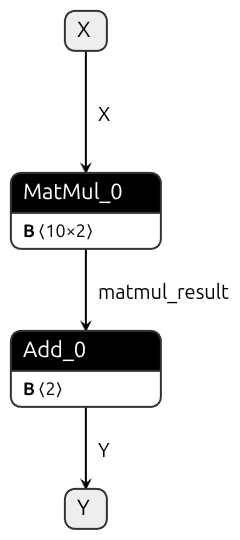
\includegraphics[height=8cm]{imgs/simple_net.onnx.png}
    \end{minipage}
    \caption{A simple VNN-LIB network declaration.}
    \label{fig:simple_net}
\end{figure}

\subsubsection*{Multiple networks}
\label{sec:multi-network-declarations}
VNN-LIB supports defining multiple networks in a single file by including multiple `(declare-network ...)` expressions. This is essential for properties that compare networks, 
such as checking for equivalence between two models or verifying properties of a composite system, like an observer-controller architecture. Figure~\ref{fig:multi_network} 
shows an example of a VNN-LIB file that declares two networks, \texttt{teacher\_net} and \texttt{student\_net}.

\begin{figure}[htbp]
    \begin{minipage}[c]{0.55\textwidth}
        \begin{lstlisting}[
            style=lbnf,
            label={lst:multi_network}
        ]
(declare-network teacher_net
    (declare-input x_teacher Real 1 32)
    (declare-output y_teacher Real 1 2)
)

(declare-network student_net
    (declare-input x_student Real 1 32)
    (declare-output y_student Real 1 2)
)
        \end{lstlisting}
    \end{minipage}
    \begin{minipage}[c]{0.45\textwidth}
        \centering
        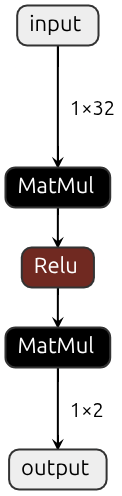
\includegraphics[height=8cm]{imgs/teacher_net.onnx.png}
        \vspace{0.5cm} 
        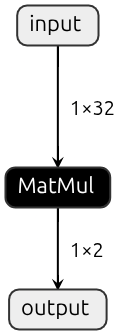
\includegraphics[height=8cm]{imgs/student_net.onnx.png}
        \label{fig:multi_network}
    \end{minipage}
    \caption{Two networks declared in VNN-LIB: \texttt{teacher\_net} and \texttt{student\_net}.}
\end{figure}

\subsubsection*{Input and Output Variable Declarations}
\label{sec:input-output-declarations}
An input variable is declared using the \texttt{declare-input} keyword, followed by a variable name, its element type (e.g., \texttt{Real}, \texttt{int8}), 
and a space-seperated list of integers representing the shape of the tensor. Similarly, an output variable uses the \texttt{declare-output} keyword. Multiple 
input and output variables can be declared within a single network declaration. There are two ways to map these declared variables to the nodes in the ONNX model:
\begin{enumerate}
    \item \textbf{Ordered Mapping (Default):} The variables are mapped to the ONNX graph's inputs/outputs based on their order of declaration. This is demonstrated in Example~\ref{lst:ordered_mapping}
    \item \textbf{Explicit Name Mapping:} Alternatively, variables can be explicitly mapped using its identifier within the ONNX graph. If this method is used, all input and output 
        variables within that network declaration must be given an explicit ONNX node name. This is demonstrated in Example~\ref{lst:named_mapping}.
\end{enumerate}

\begin{figure}[htbp]
    \centering
    \begin{lstlisting}[
        caption={A network with multiple inputs/outputs, mapped by declaration order.},
        style=lbnf,
        label={lst:ordered_mapping}
    ]
(declare-network multi_io_net
    (declare-input image Real 1 3 224 224)
    (declare-input metadata Real 1 10)
    (declare-output logits Real 1 1000)
    (declare-output bbox Real 1 4)
)
    \end{lstlisting}
    \begin{lstlisting}[
        caption={The same network, but with explicit ONNX node name mapping.},
        style=lbnf,
        label={lst:named_mapping}
    ]
(declare-network multi_io_net
    (declare-input image Real 1 3 224 224 onnx-node:"image")
    (declare-input metadata Real 1 10 onnx-node:"metadata")
    (declare-output logits Real 1 1000 onnx-node:"logits")
    (declare-output bbox Real 1 4 onnx-node:"bbox")
)
    \end{lstlisting}
    \vspace{0.5cm}
    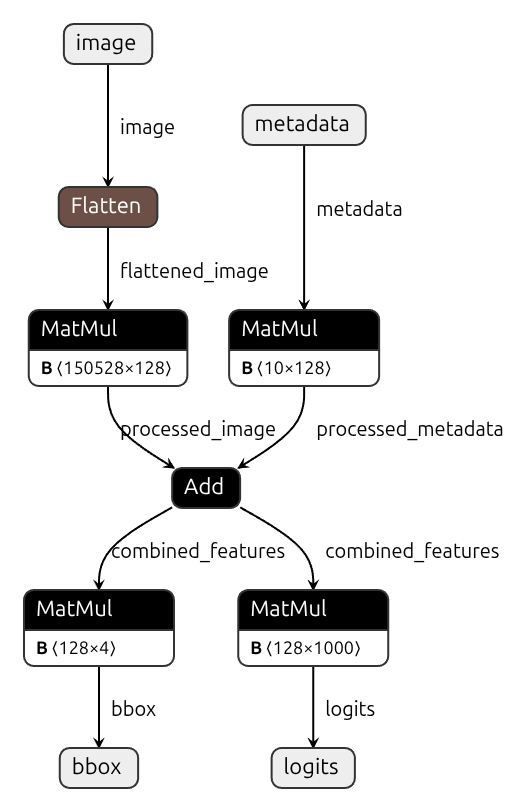
\includegraphics[height=10cm]{imgs/multi_io_net.onnx.png}
    \caption{A VNN-LIB network declaration with multiple inputs and outputs. The first example uses ordered mapping, while the second uses explicit ONNX node names.}
    \label{fig:multi_io_net}
\end{figure}

\subsubsection*{Hidden Node Declarations}
\label{sec:hidden-node-declarations}
A hidden node is declared using the \texttt{declare-hidden} keyword. This declaration includes a variable name for use within the VNN-LIB specification, 
its element type, its tensor shape, and crucially, a string identifier that specifies the corresponding node name in the ONNX graph. The ability to declare hidden nodes
allows for properties to reference key intermediate computations within the network, such as encoding features, attention mechanisms, or other internal states. Multiple
hidden nodes can be trivially declared within a single network declaration. Figure~\ref{fig:hidden_node} shows an example of a VNN-LIB network declaration with a hidden node.

\begin{figure}[htbp]
    \begin{minipage}[c]{0.55\textwidth}
        \begin{lstlisting}[
            style=lbnf,
            label={lst:hidden_node}
        ]
(declare-network encoder
    (declare-input X Real 1 28 28)
    (declare-hidden feature_embedding Real 1 128 onnx-node:"encoder_layer4/output")
    (declare-output Y Real 1 10)
)
        \end{lstlisting}
    \end{minipage}%
    \begin{minipage}[c]{0.45\textwidth}
        \centering
        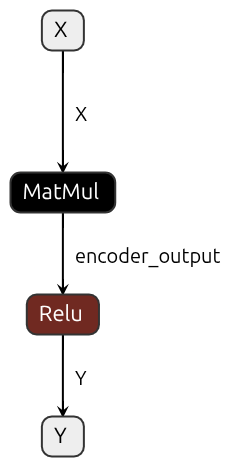
\includegraphics[height=8cm]{imgs/encoder_net.onnx.png}
    \end{minipage}
    \caption{A VNN-LIB network declaration with a hidden node. The hidden node \texttt{feature\_embedding} corresponds to the ONNX node \texttt{encoder\_layer4/output}.}
    \label{fig:hidden_node}
\end{figure}

\subsubsection*{Assertion declarations}
\label{sec:assertion-declarations}
VNN-LIB supports quantifier-free logical formulas as \textit{assertions}. Assertions are defined using parenthesized \texttt{(assert\ldots)} expressions, and following an SMT-LIB-like syntax with the 
operator preceding its operands. An assertion is a logical formula that may include logical connectives, relational comparisons, and arithmetic expressions over declared tensors and constants.

\subsubsection*{Variables and Indexing}
\label{sec:variables-and-indexing}
Assertions may only refer to individual elements of declared tensors. To refer to a specific scalar element within a tensor, an indexing notation is used. Let $X \in I$ be an $n$-dimensional tensor 
in some generic input domain $I = I^{d_1 \times \cdots \times d_n}$. The ``matrix notation'' represents a specific element $x_{i_1, i_2, \dots, i_n}$ of the tensor $X$ as \texttt{X[$i_1$,$i_2$,\dots,$i_n$]}, 
where $i_1, \dots, i_n$ are zero-based indices ranging from $0$ to $d_1{-}1$, $0$ to $d_2{-}1$, \dots, $d_n{-}1$, respectively. To better clarify, if we consider the 1-D tensor $X \in I^n$, the 2-D tensor 
$Y \in I^{n \times m}$, and the 3-D tensor $Z \in I^{n \times m \times p}$, we will have the following representations:
\begin{itemize}
    \item \texttt{X[0]}, \texttt{X[1]}, \dots, \texttt{X[$i$]}, \dots, \texttt{X[$n$]};
    \item \texttt{Y[0,0]}, \texttt{Y[0,1]}, \dots, \texttt{Y[$i$,$j$]}, \dots, \texttt{Y[$n$,$m$]};
    \item \texttt{Z[0,0,0]}, \texttt{Z[0,0,1]}, \dots, \texttt{Z[$i$,$j$,$k$]}, \dots, \texttt{Z[$n$,$m$,$p$]};
\end{itemize}
In such a representation, \texttt{Z[$i$-$j$-$k$]} corresponds to the element $z_{i,j,k}$ of the tensor $Z$. 

\subsubsection*{Arithmetic expressions}
Arithmetic expressions are formed using prefix notation with the following supported operators:
\begin{itemize}
    \item \texttt{(+ a b ...)}: Addition of two or more terms. 
    \item \texttt{(- a b ...)}: Subtraction of two or more terms. Alternatively, \texttt{(- a)} for negation.
    \item \texttt{(* a b ...)}: Multiplication of two or more terms. 
\end{itemize}
Operands (\texttt{a}, \texttt{b},...) can be constants, indexed tensors, or other nested arithmetic expressions.

\subsubsection*{Boolean expressions}
Boolean expressions are defined as expressions that produce a Boolean (\texttt{true} or \texttt{false}) value. They are formed using comparison operators and logical connectives:
\begin{itemize}
    \item \textbf{Comparison Operators:} \texttt{<=}, \texttt{>=}, \texttt{<}, \texttt{>}, \texttt{=}, \texttt{!=}
    \begin{itemize}
        \item The operands may be constants, indexed tensors, or arithmetic expressions. Each operator has two operands.
        \item For example \texttt{(<= a b)} returns true if $a$ is less than or equal to $b$.
    \end{itemize}
    \item \textbf{Logical Connectives:} \texttt{and}, \texttt{or}
    \begin{itemize}
        \item The operands must be Boolean expressions. Each operator can take two or more operands.
        \item For example \texttt{(and a b ...)} returns true if all operands are true.
    \end{itemize}
\end{itemize}

\subsection*{Assertion Example}
\begin{lstlisting}[
    caption={An assertion stating that if the input $A_0$ is between 0 and 1, the output $B_0$ must be greater than $B_1$ and their sum must be non-negative.},
    style=lbnf,
    label={lst:assertion-example}
]
(assert
    (and
        (and (>= A_0 0.0) (<= A_0 1.0))
        (and (> B_0 B_1) (>= (+ B_0 B_1) 0.0))
    )
)
\end{lstlisting}

\section{Scoping}
\label{sec:scoping}

TODO Ann

\section{Typing}
\label{sec:typing}

TODO Ann

\section{Semantics}
\label{sec:semantics}

TODO Ann

